% perk
\begin{frame}{Signal Model}
	\uncover<+->{%
		\textbf{Given}: at every voxel, measurement vector $\bmy \in \complexes{D}$ modeled as 
		\begin{align}
			\bmy = \bms\paren{\bmx,\bmnu} + \bmeps
			\label{eq:model}
		\end{align}
		\begin{itemize}
			\item{\makebox[3cm][l]{$\bmx \in \reals{L}$} unknown parameters}
			\item{\makebox[3cm][l]{$\bmnu \in \reals{K}$} ``known'' parameters}
			\item{\makebox[3cm][l]{$\bms : \reals{L+K} \mapsto \complexes{D}$} 
				vector signal model}
			\item{\makebox[3cm][l]{$\bmeps \in \complexes{D}$} 
				noise $\sim \cgauss{\zeros{D}}{\bmSig}$
			}
		\end{itemize}
		\vspace{0.5cm}
	}
	\uncover<+->{%
		\textbf{Task}: design fast voxel-by-voxel estimator $\esta{\bmx}{\bmy,\bmnu}$
	}
\end{frame}

\begin{frame}{Prior Work}
	\uncover<1->{%
		\textbf{Task}: design fast voxel-by-voxel estimator $\esta{\bmx}{\bmy,\bmnu}$
  	
  	\textbf{Challenges}:
  	\begin{itemize}
  		\item{signal $\bms$ often nonlinear in $\bmx$: non-convex inverse problems}
  		\item{signal $\bms$ might be difficult to write in closed form}
  	\end{itemize}
	}
	\uncover<2->{%
  	\textbf{Conventional Approaches:}
	}
  	\begin{itemize}
			\item<2-3>{gradient-based local optimization}
			\begin{itemize}
				\item{initialization-dependent solution}
				\item{requires signal gradients}
			\end{itemize}
  		\item<3>{stochastic methods (\eg, simulated annealing)}
  		\begin{itemize}
  			\item{unclear convergence analysis \hfill \citec{bertsimas:93:sa}}
  			\item{several unintuitive tuning parameters}
  		\end{itemize}
		\item<4>{%
			dictionary-based grid search
		}
  	\end{itemize}
\end{frame}

\begin{frame}{Motivation}
	\textbf{Grid search} computational costs
	\begin{table}
		\centering
		\begin{tabular}{r|cc}
			& $L$ & $\sim$number dictionary atoms \\
			\hline
			\uncover<1-2>{1-compartment relaxivity 		& 3 		& $\sim$$100^2$ \\}
			\uncover<2>{flow velocity 									& 4 		& $\sim$$100^3$ \\} 
			\uncover<2>{diffusivity tensor 							& 7 		& $\sim$$100^6$ \\}
			\uncover<2->{\hlg{2-3 compartment relaxivity}& 6-10 	& $\sim$$100^5-100^9$} 
			\end{tabular}
		\end{table}
		
		\uncover<3>{
			\textbf{Can we scale computation with $L$ more gracefully?}
		}
\end{frame}

\begin{frame}{Machine Learning for QMRI Parameter Estimation}
	\uncover<1->{%
		\textbf{Idea}: learn a \emph{nonlinear} estimator from simulated training data
	}
	\begin{itemize}
		\item<2-3>{%
			sample $\paren{\bmx_1,\bmnu_1,\bmeps_1},\dots,\paren{\bmx_N,\bmnu_N,\bmeps_N}$
			from prior distributions
		}
		\item<2-3>{%
			simulate image data vectors $\bmy_1,\dots,\bmy_N$ 
			via signal model $\bms$
		}
		\item<3-5>{%
			design \emph{nonlinear} functions $\est{x}_l\paren{\cdot} := \est{h}_l\paren{\cdot} + \est{b}_l$ 
			for $l \in \set{1,\dots,L}$ \\
			that map each $\bmq_n := [\re{\bmy_n}\tpose, \im{\bmy_n}\tpose, \bmnu_n\tpose]\tpose \in \setQ$	
			to $x_{l,n} \in \real$
		}
	\end{itemize}	
	\vspace{-0.3cm}
	\uncover<4->{%
		\alt<4-5>{%
			\begin{align}
				\paren{\est{h}_l,\est{b}_l} \in \set{
					\argmin{\substack{h_l \\ b_l \in \real}} 
					\frac{1}{N} \sum_{n=1}^N \paren{h_l\paren{\bmq_n} + b_l - x_{l,n}}^2
				}
				\uncover<5>{
					\,\,\,\,\, \textcolor{red}{\text{ill-posed!}}
				}
				\nonumber
			\end{align}
		}{%
			\begin{align}
				\paren{\est{h}_l,\est{b}_l} \in \set{
					\argmin{\substack{h_l \hlb{\in \hilb} \\ b_l \in \real}}
					\frac{1}{N} \sum_{n=1}^N \paren{h_l\paren{\bmq_n} + b_l - x_{l,n}}^2
					\hlb{+ \rho_l \norm{h_l}^2_\hilb}
				}
				\label{eq:krr,cost}
			\end{align}
		}
	}
	\uncover<6->{%
		\textbf{Solution}: Parameter Est. via Regression with \hlm{Kernels} (PERK) \\
			\hfill \citec{nataraj::dfm}
		\begin{itemize}
			\item{restrict optimization to a \hlb{certain rich function space $\hilb$}}
			\item{optimal $\est{h}_l \hlb{\in \hilb}$ takes form 
				$\est{h}_l = \sum_{n=1}^N \est{a}_{l,n} \hlm{k}(\cdot,\bmq_n)$ \\
				\hfill \citec{scholkopf:01:agr}}
		\end{itemize}
	}	
\end{frame}

\begin{comment}
\begin{frame}{A Function Space over which Optimization is Tractable}
	\uncover<1>{%
		\textbf{Hilbert space}: complete inner product function space
		\vspace{0.5cm}
	}
	\uncover<2->{%
  	\hlb{\textbf{Reproducing kernel Hilbert space (RKHS)}} \\
  	Hilbert space $\hlb{\hilb}$ over input space $\setQ$ with \emph{reproducing property}
  	$$\innprod{h}{\hlm{k}(\cdot,\bmq)}_{\hlb{\hilb}} = h(\bmq), 
  		\qquad \forall h \in \hlb{\hilb}, \bmq \in \setQ$$ 
  	for some $\hlm{k} : \setQ^2 \mapsto \real$ called a \hlm{reproducing kernel (RK)} \\
  	\vspace{0.5cm}
	}
  \uncover<3->{%
  	\textbf{Relevant facts}
  	\begin{itemize}
  		\item{Bijection between RKHS $\hlb{\hilb}$ and RK $\hlm{k}$ 
  			\hfill \citec{aronszajn:50:tor}}
			\item{Function $\hlm{k}(\cdot,\bmq) \in \hlb{\hilb}$ 
  			called a \emph{feature mapping}}
  	\end{itemize}
	}
\end{frame}

\begin{frame}{Function Optimization over a RKHS}
	\uncover<1-3>{%
		\textbf{Choose}: RK $\hlm{k} : \setQ^2 \mapsto \real$, 
			which induces choice of RKHS $\hlb{\hilb}$ 
	}
	\only<2>{%
		\begin{itemize}
			\item{\emph{Nonlinear} kernel corresponds to \emph{nonlinear} estimation}
			\item{We use $\hlm{k}(\bmq,\bmq') \gets \expa{-\frac{1}{2}\norm{\bmL^{-1}\paren{\bmq-\bmq'}}_2^2}$}
		\end{itemize}
	}
	\uncover<3->{%
		\textbf{Solve}: for each desired latent parameter $l \in \set{1,\dots,L}$,
		\begin{align}
			\paren{\est{h}_l,\est{b}_l} \in 
				\set{\argmin{\substack{h_l \in \hlb{\hilb} \\ b_l \in \real}}
				\frac{1}{N} \sum_{n=1}^N \paren{h_l\paren{\bmq_n} + b_l - x_{l,n}}^2
				+ \rho_l \norm{h_l}^2_{\hlb{\hilb}}}
			\label{eq:krr,cost}
		\end{align}
	}
	\begin{itemize}
		\item<4->{%
			Optimal $\est{h}_l$ over $\hlb{\hilb}$ takes form \hfill \citec{scholkopf:01:agr}
			\begin{align}
				\est{h}_l\paren{\cdot} \equiv \sum_{n=1}^N \est{a}_{l,n} \hlm{k}\paren{\cdot,\bmq_{n}}
				\label{eq:gen-rep}
			\end{align}
		}
  	\item<5->{%
  		Plug \eqref{eq:gen-rep} into \eqref{eq:krr,cost}; 
  			solve now instead for $\paren{\est{a}_l,\est{b}_l}$; construct:
  		\begin{align}
  			\est{x}_l\paren{\cdot} = 	
  				\sum_{n=1}^N \est{a}_{l,n} \hlm{k}\paren{\cdot,\bmq_n} + \est{b}_l
  			\label{eq:krr,sol}
  		\end{align}
  	}
	\end{itemize}
\end{frame}
\end{comment}

\begin{frame}{PERK Solution}
	Non-iterative closed-form solution, for $l \in \set{1,\dots,L}$: 
	\begin{align}
		\est{x}_l\paren{\cdot} = \bmxg{l}\tpose\paren{
			\frac{1}{N}\ones{N} 
			+ \bmM\inv{\bmK\bmM + N\rho_l \eye{N}} 
			\paren{\bmka{\cdot} - \frac{1}{N}\bmK\ones{N}}
		}
		\label{eq:krr,x-hat}
	\end{align}
	\begin{itemize}
	\item<1-4>{%
		\makebox[6cm][l]{$\bmxg{l} := [x_{l,1},\dots,x_{l,N}]\tpose$}
		training pt regressands
	}
	\item<2-4,6>{%
		\makebox[6cm][l]{%
			$\bmK := 
				\begin{bmatrix}
					\hlm{k}(\bmq_1,\bmq_1) 	& \cdots 	& \hlm{k}(\bmq_1,\bmq_N) \\
					\vdots									& \ddots	& \vdots \\
					\hlm{k}(\bmq_N,\bmq_1) 	& \cdots 	& \hlm{k}(\bmq_N,\bmq_N)
				\end{bmatrix}$
		}
		Gram matrix
	}						
	\item<3-4>{%
		\makebox[6cm][l]{$\bmM := \eye{N} - \frac{1}{N}\ones{N}\ones{N}\tpose$}
		de-meaning operator
	}
	\item<4>{%
		\makebox[6cm][l]{%
			$\bmka{\cdot} := \brac{\hlm{k}(\cdot,\bmq_1),\dots,\hlm{k}(\cdot,\bmq_N)}\tpose$
		}
		nonlin kernel embedding
	}
	\end{itemize}
	\uncover<5>{%
		Can we scale computation with $L$ more gracefully?
	}
	\begin{itemize}
		\item<5>{Yes, in fact \eqref{eq:krr,x-hat} separable in $l \in \set{1,\dots,L}$ by construction}
		\item<6>{However, explicitly computing $\bmK$ may be undesirable...}
	\end{itemize}
\end{frame}

\begin{frame}{PERK as High-Dimensional Affine Regression}
	\uncover<1->{
		Suppose there exists``approximate feature mapping'' $\bmztZ : \setQ \mapsto \reals{Z}$ \\
		such that $\bmZt := \brac{\bmztZa{\bmq_1},\dots,\bmztZa{\bmq_N}}$ has for $\dim\paren{\setQ} \ll Z \ll N$
		\begin{align}
			\bmK \approx \bmZt\tpose \bmZt.
			\label{eq:low-rank}
		\end{align}
		\vspace{-0.5cm}
	}
	\uncover<2-3>{%
		\begin{overlayarea}{\textwidth}{2.5cm}
  		\alt<2>{%
    		Plugging \eqref{eq:low-rank} into KRR solution \eqref{eq:krr,x-hat} and rearranging gives
    		\begin{align}
    			\est{x}_l\paren{\cdot} \approx 
    				\frac{1}{N}\bmxg{l}\tpose\ones{N} 
    				+ \frac{1}{N}\bmxg{l}\tpose \bmM \bmZt\tpose
    				\inv{\frac{1}{N} \bmZt \bmM \bmZt\tpose + \rho_l\eye{Z}}
    				\paren{\bmztZa{\cdot}-\frac{1}{N}\bmZt\ones{N}}
    				\nonumber
    		\end{align}
    	}{%
    		Plugging \eqref{eq:low-rank} into KRR solution \eqref{eq:krr,x-hat} and rearranging gives
    		\begin{align}
    			\est{x}_l\paren{\cdot} \approx 
    				\mxl + \cxlzt \inv{\Cztzt + \rho_l\eye{Z}} \paren{\bmztZa{\cdot} - \bmmzt}
    				\label{eq:x-cme}
    		\end{align}
				which is regularized $Z$-dimensional affine regression!
    	}
		\end{overlayarea}
	}
	\uncover<4->{%
		Does such a $\bmzt$ exist and work well in practice?
		\begin{itemize}
			\item{Yes, \eg for Gaussian
				$\hlm{k}(\bmq,\bmq') \gets \expa{-\frac{1}{2}\norm{\bmL^{-1}\paren{\bmq-\bmq'}}_2^2}$ \\
				\hfill \citec{rahimi:07:rff}}
			\item{In such cases, can reduce from $\sim$$N^2$ to $\sim$$NZ$ computations}
		\end{itemize}
	}
\end{frame}

\begin{comment}
\begin{frame}{Model Selection}
	\uncover<1-7>{%
		\emph{Online} model selection: train \emph{after} observing (unlabeled) test data
		\begin{itemize}
			\item<2>{\makebox[6cm][l]{Prior on known $\bmnu$} 
				density estimation}
			\item<2>{\makebox[6cm][l]{Noise covariance $\bmSig$}
				low-signal data regions}
			\item<3-6>{%
				\alt<1-6>{%
					\makebox[6cm][l]{Regularization parameters} Bayesian perspective...
				}{%
					\makebox[6cm][l]{Regularization parameters}
						$\rho_l \gets \frac{1}{N^2}\bmxg{l}\tpose\bmM\bmxg{l}$
				}
  			\begin{itemize}
  				\item<4>{%
  					Assume prior 
  					$h_l\paren{\cdot} + b_l \sim \GP{0\paren{\cdot}}{\hlm{k}\paren{\cdot,\cdot}},
  					l \in \set{1,\dots,L}$
  				}
  				\item<5>{%
  					Include latent parameter variability $\epsilon_{x_l}$ \\
  					in observed regressand model 
						$x_l\paren{\bmq} = h_l\paren{\bmq} + b_l + \epsilon_{x_l}$
  				}
  				\item<6>{%
  					If we further assume $\epsilon_{x_l} \sim \gauss{0}{N\rho_l}$
  					then posterior mean function is KRR solution \eqref{eq:krr,x-hat}
  					\hfill \citec{rasmussen:05:gpf}
  				}
  				\item<6>{%
  					Reasonable to set 
  					$N\rho_l \gets \cov{x_l} \approx \frac{1}{N} \bmxg{l}\tpose\bmM\bmxg{l}$
  				}
  			\end{itemize}
			}
			\item<7>{%
				\makebox[6cm][l]{Kernel smoothing length-scale}
				$\bmL \gets \diag{\sum_{n=1}^N \bmq_n}$
			}
		\end{itemize}
	}
	\uncover<8->{%
		Some parameters still require manual selection...
		\begin{itemize}
			\item{%
				\makebox[3cm][l]{Prior on $\bmx$}
				from tissue properties
			}
			\item{%
				\makebox[3cm][l]{Kernel shape}
				$k(\bmq,\bmq') \gets \expa{-\frac{1}{2}\norm{\bmL^{-1}\paren{\bmq-\bmq'}}_2^2}$
			}
		\end{itemize}
	}
\end{frame}
\end{comment}

\begin{frame}{Experimental Setup}
	\uncover<1->{%
		Demonstrated PERK for $\To,\Tt$ est from optim (2SP,1DE) scan
	}%
	\begin{itemize}
		\item<2>{%
			PERK trained using $N \gets 10^6$ samples from prior dist $\dist{\bmx,\bmnu}$
		}%
		\item<2>{%
			To enable precise estimation,
			support of $\dist{\bmx,\bmnu}$ carefully chosen \\
			to coincide with min-max acquisition design support
		}%
	\end{itemize}
	
	\uncover<3->{%
		Compared PERK estimates to grid search estimates \\
		via variable projection method (VPM) \hfill{\citec{golub:03:snl}}
	}%
\end{frame}
	
\begin{frame}{Phantom Results}
	\uncover<1->{%
  	\begin{figure}
  		\centering
  		\subfloat{%
				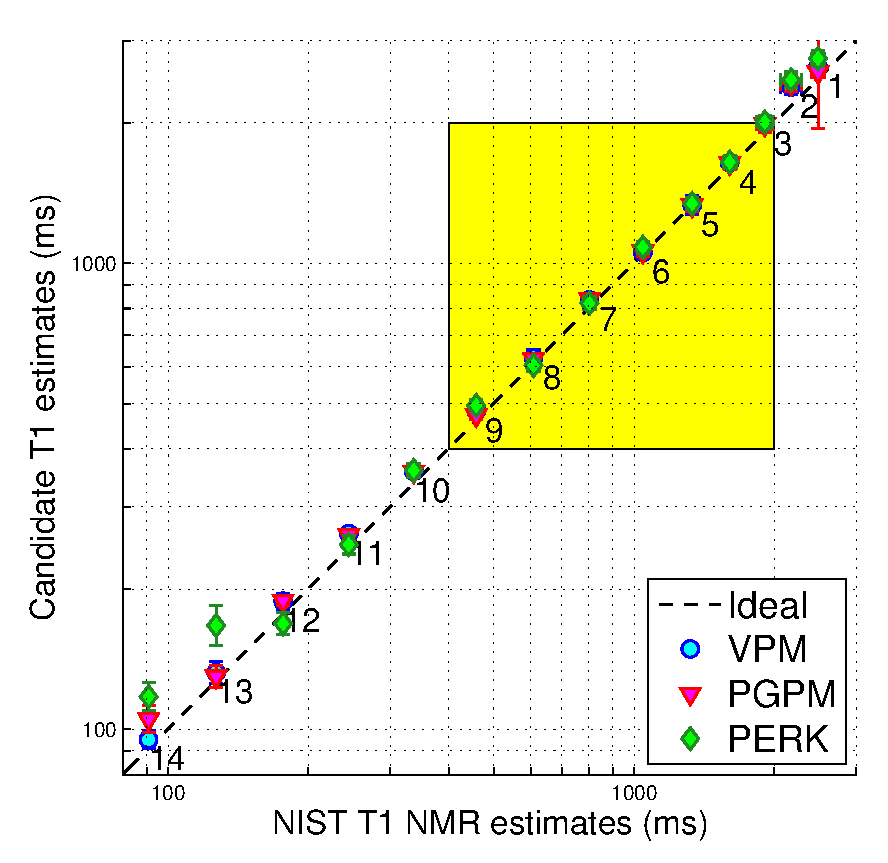
\includegraphics [width=0.45\textwidth] 
          {hpd-tight/sp2de1,sl-6,t1,plot.eps}
        \label{fig:perk,hpd,t1}
      }%
      \hspace{0.3cm}
      \subfloat{%
      	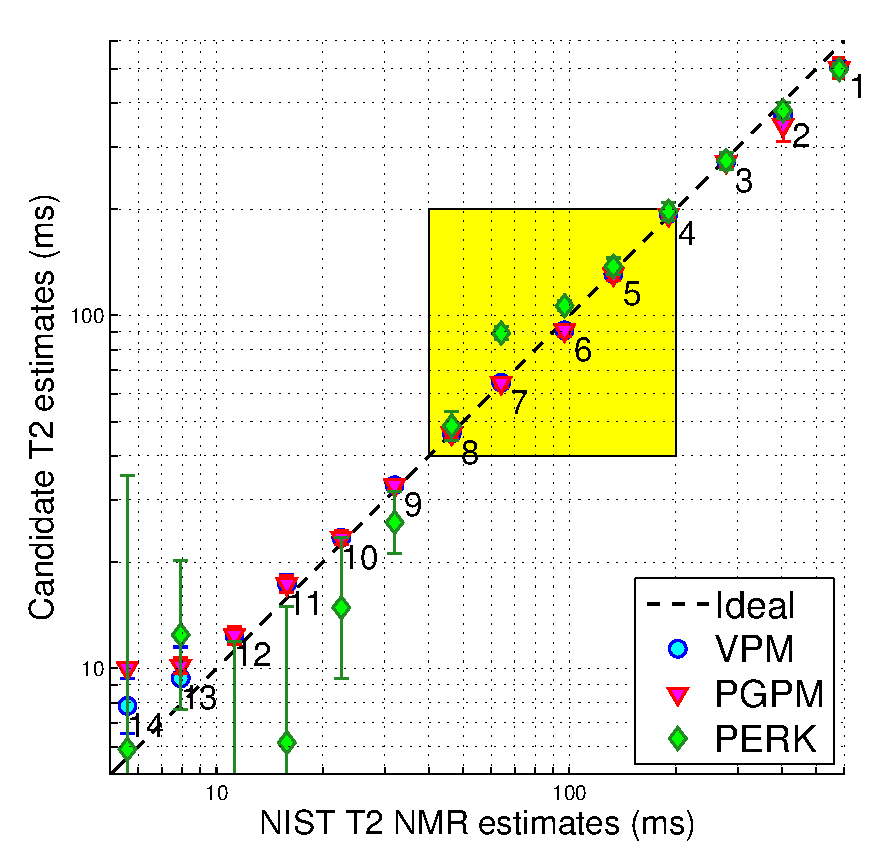
\includegraphics [width=0.45\textwidth] 
					{hpd-tight/sp2de1,sl-6,t2,plot.eps}
				\label{fig:perk,hpd,t2}
      }%
      \label{fig:perk,hpd}
   	\end{figure}
	}%
	\uncover<2->{%
		Within support of $\dist{\bmx,\bmnu}$, \\
		\textbf{PERK and grid search estimates agree excellently}.
	}%
\end{frame}

\begin{frame}{\emph{In vivo} Results}
	\vspace{-0.3cm}
	\uncover<1->{%
  	\begin{figure}
  		\subfloat{
  			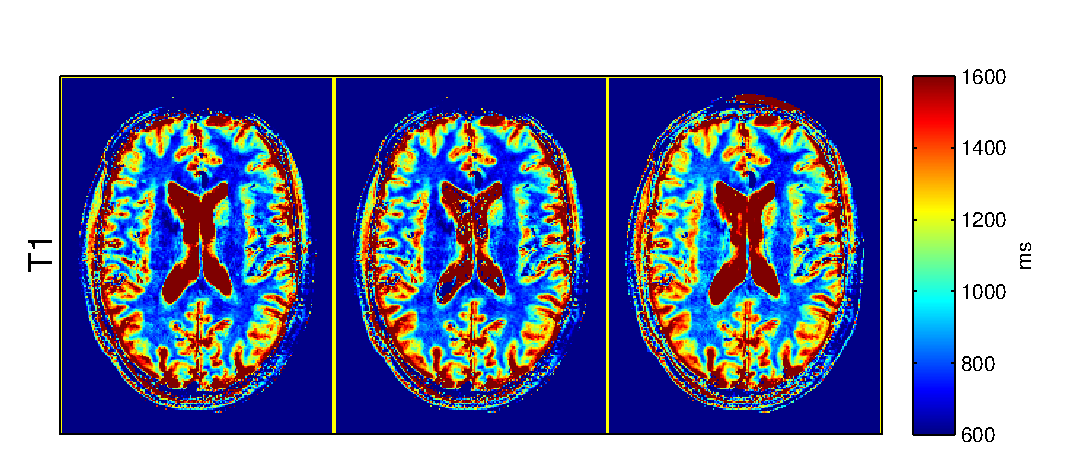
\includegraphics [width=0.58\textwidth,clip] 
  				{s,perk/sp2de1,sl-5,t1,im-jet.eps}
  			\label{fig:perk,brain,t1}
  		}
  		\vspace{0cm}
  		\subfloat{
  			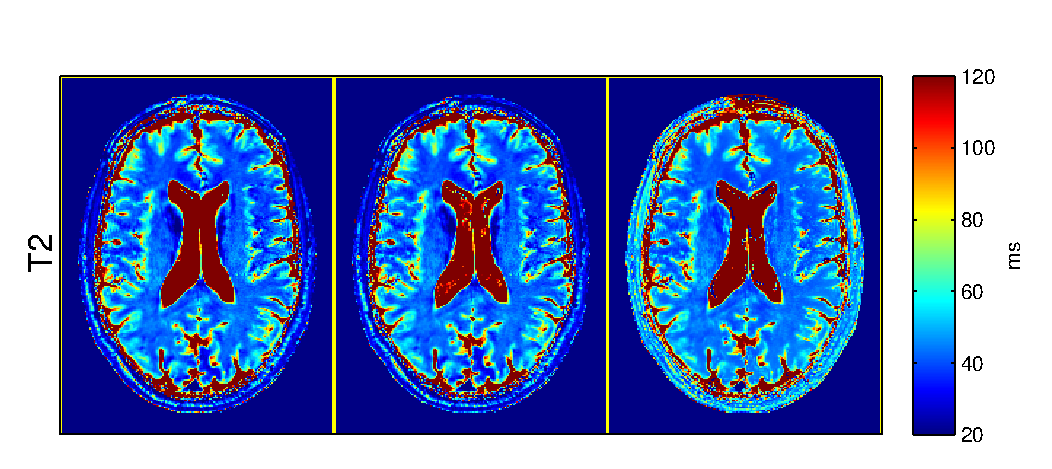
\includegraphics [width=0.57\textwidth,clip]
  				{s,perk/sp2de1,sl-5,t2,im-jet.eps}
  			\label{fig:perk,brain,t2}
  		}
  		\label{fig:perk,brain}
  	\end{figure}
	}%
	\vspace{-0.3cm}
	\uncover<2->{%
		\makebox[4.2cm][r]{$837$s}
		\makebox[3.5cm][r]{$32$s train, $1.6$s test}
	}	
\end{frame}

\begin{frame}{Summary}
	\uncover<1->{%
		\textbf{Contributions}
		\begin{itemize}
			\item<1->{\textbf{PERK}: fast, dictionary-free ML method for QMRI}
			\item<2->{demonstrated PERK for $\To,\Tt$ estimation}
			\begin{itemize}
				\item<2>{%
					Phantom (and omitted simulation) results show that \\
					PERK and grid search yield comparable accuracy and precision
				}
				\item<2>{%
					\emph{In vivo} PERK and grid search estimates are comparable
				}
				\item<2-3>{%
					\textbf{PERK is consistently at least $23$x faster}
				}
			\end{itemize}
		\end{itemize}
	}
	\uncover<3>{%
		\textbf{Can we exploit PERK's speed in a more compelling problem?}
	}
\end{frame}
